\documentclass{beamer}

\usetheme{zg}

\title{RESTful API}
\date{\today}
\author{Fernando Camargo}
\institute{ZG Soluções}


\begin{document}
\maketitle

\section{Por que REST?}

\begin{frame}{Web App vs Web Service}
  \begin{outline}
    \1<1-> Aplicações Web convencionais
  \0 \visible<1->{\resizebox{!}{1in}{\includesvg{Web-Applications}}}
    \1<2-> Web Services
  \0 \visible<2->{\resizebox{!}{1in}{\includesvg{Web-Services}}}
  \end{outline}
\end{frame}

\begin{frame}{Menor gasto de rede}
  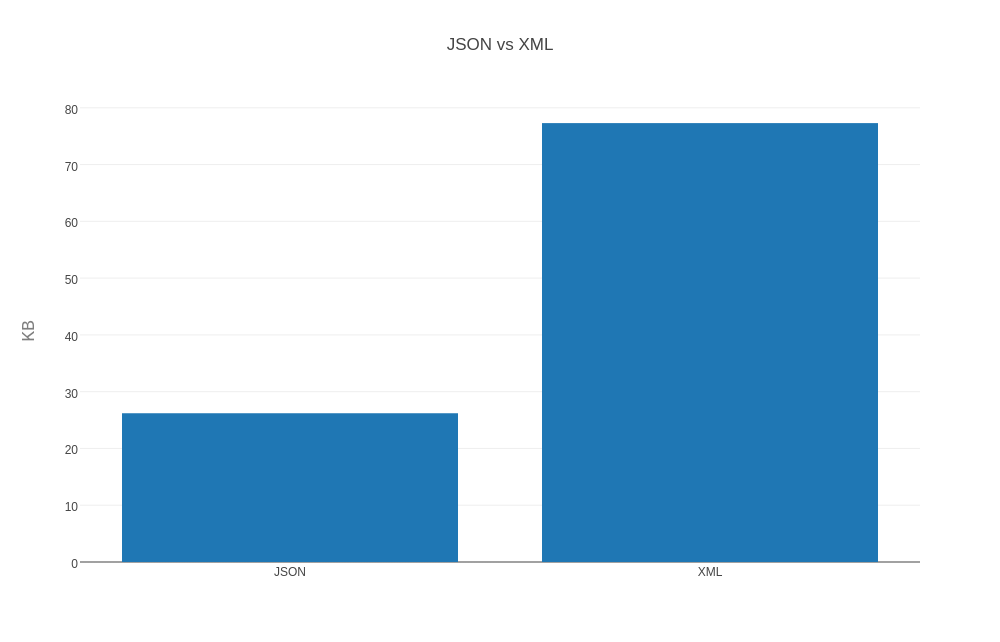
\includegraphics[width=\textwidth]{JSON-vs-XML}\\
  {\tiny Fonte: \cite{davelaar2015}}
\end{frame}

\begin{frame}{Melhor performance}
  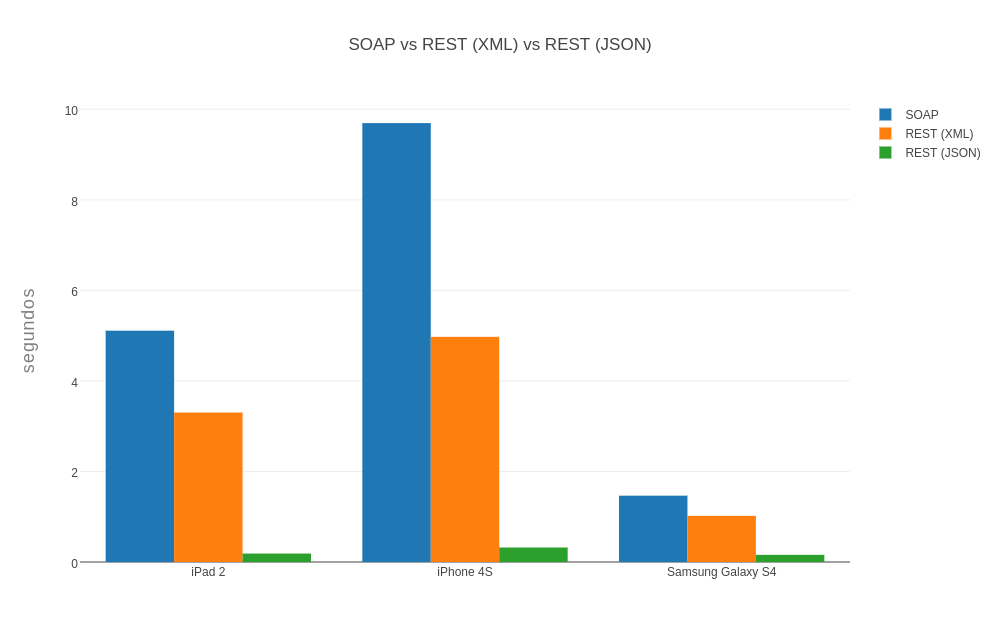
\includegraphics[width=\textwidth]{SOAP-vs-REST}\\
  {\tiny Fonte: \cite{davelaar2015}}
\end{frame}


\begin{frame}{SOAP vs REST}
  \begin{table}[]
    \begin{tabular}{@{}ll@{}}
      \toprule
      \textbf{SOAP}                       & \textbf{REST}                           \\ \midrule
      Especificação                       & Padrão arquitetural                     \\ \pause
      Projetado para \alert{servidores}   & Projetado para \alert{clientes leves}   \\ \pause
      Stateful                            & Stateless                               \\ \pause
					  & Possibilita cache                       \\ \pause
      Baseado em ações                    & Baseado em recursos                     \\ \bottomrule
    \end{tabular}
  \end{table}
\end{frame}

\section{Padrão Arquitetural do REST}

\begin{frame}{Regras}
  \begin{outline}
    \1<1-> Inferface Uniforme
    \1<2-> Stateless
    \1<3-> Cacheable
    \1<4-> Cliente-Servidor
      \2 Servidor: armazenamento de dados
      \2 Cliente: apresentação e manutenção de sessão
    \1<5-> Sistema em Camadas (possibilidade)
    \1<6-> Código sob Demanda (possibilidade)
  \end{outline}
\end{frame}

\subsection{Inferface Uniforme}

\begin{frame}{Interface Uniforme}
  \begin{outline}
    \1<1-> Baseada em \alert{recursos}
    \1<2-> Recursos identificados por URL
    \1<3-> Ações por métodos HTTP
    \1<4-> URLs com substantivos no plural
  \end{outline}
\end{frame}

\begin{frame}{URLs Incorretas}
  \begin{outline}
    \1 /listarProdutos
    \1 /obterProdutos/1
    \1 /criarProdutos
    \1 /deletarProdutos/1
  \end{outline}
\end{frame}

\begin{frame}{URLs Corretas}
  \begin{outline}
    \1 /produtos
    \1 /produtos/1
  \end{outline}
\end{frame}

\begin{frame}{Interface Uniforme}
  \begin{outline}
    \1<1-> \textbf{Re}presentational \textbf{S}tate \textbf{T}ransfer
    \1<2-> \textbf{HATEOAS}: \textbf{H}ypermedia \textbf{a}s \textbf{t}he \textbf{E}ngine \textbf{o}f \textbf{A}pplication \textbf{S}tate 
    \1<3-> Mensagens autodescritivas
  \end{outline}
\end{frame}

\subsection{Protocolo HTTP}

\begin{frame}{Métodos HTTP}
  \begin{table}[]
  \begin{tabular}{@{}lll@{}}
  \toprule
  Método & Ação                                   & Idempotente \\ \midrule
  GET    & Obtenção                               & Sim         \\ \pause
  HEAD   & Obtenção de metadados                  & Sim         \\ \pause
  DELETE & Remoção                                & Sim         \\ \pause
  POST   & Criação sem ID ou atualização parcial  & Não         \\ \pause
  PUT    & Criação com ID ou atualização completa & Sim         \\ \bottomrule
  \end{tabular}
  \end{table}
  {\tiny Idempotência: múltiplas requisições não alteram o resultado}
\end{frame}

\begin{frame}{Status HTTP}
  \begin{outline}
    \1<1-> 200 OK
    \1<2-> 201 Created
    \1<3-> 304 Not Modified
    \1<4-> 400 Bad Request
    \1<5-> 401 Unauthorized
    \1<6-> 403 Forbidden
    \1<7-> 404 Not Found
  \end{outline}
\end{frame}

\section{Boas Práticas}

\begin{frame}{Versionamento}
  
\end{frame}


\begin{frame}[allowframebreaks]{Referências}
  %\nocite{*} % Se quiser que todas citações apareçam
  \bibliography{./bib/rest.bib}
\end{frame}

\end{document}
